\chapter{Método de Trabajo}
\label{chap:metodo}

\drop{E}{n} este capítulo se expone la metodología de trabajo utilizada en el proyecto, Scrum. Además,
se exponen las herramientas utilizadas para elaborar el \acs{TFG}.

\section{Scrum}

Scrum~\cite{SCRUM}~\cite{SCRUMXP} es un marco de trabajo donde se pueden emplear diferentes procesos y técnicas. Inicialmente 
fue ideado para gestionar y desarrollar productos, pero se puede encontrar equipos utilizando Scrum 
en multitud de ámbitos como en desarrollos de software, hardware, vehículos, escuelas y en casi cualquier 
cosa.

Se emplea un desarrollo iterativo e incremental para realizar mejores estimaciones y controlar 
los riesgos. Los equipos Scrum son pequeños, flexibles y adaptativos. 

\subsection{Equipo y roles}

El equipo Scrum lo forman un Product Owner o propietario del producto, un equipo de desarrolladores y el Scrum Master. Algunas
de las características de los equipos Scrum son:

\begin{itemize}
	\item Son auto-organizados y multifuncionales.
	\item Eligen la mejor forma de llevar a cabo su trabajo y no los dirige ninguna persona externa al equipo.
	\item Los equipos tienen todas las competencias y habilidades necesarias para llevar a cabo el trabajo,
	sin necesitar personas externas al equipo.
	\item Están diseñados para optimizar la flexibilidad, la creatividad y la productividad.
	\item Entregan los productos de forma iterativa e incremental, facilitando la retroalimentación. Cada versión entregada
	es funcional y útil para el Product Owner.
\end{itemize}

\subsubsection{Product Owner}

Es el propietario del producto que desarrolla el equipo, es el responsable de trasladar al equipo el punto de vista del cliente y maximizar
el valor del producto que se esta desarrollando. Además, es la única persona responsable de gestionar la Pila del producto (Product Backlog), 
esta gestión incluye:

\begin{itemize}
	\item Expresar de forma clara las historias de usuario.
	\item Priorizar los elementos de la Pila del producto para alcanzar los objetivos.
	\item Mantener la Pila del producto visible, transparente y clara, debe mostrar lo que el equipo hará a continuación.
	\item Asegurar que el equipo entienda los elementos de la Pila del producto al nivel necesario.
\end{itemize}

\subsubsection{Equipo de desarrollo}

El equipo de desarrolladores es un grupo de personas que realizan el trabajo necesario para cumplir con las
necesidades plasmadas en las historias de usuario del Sprint Backlog(historias de usuario del sprint). Al final 
del sprint deben entregar un trabajo terminado que pueda ser puesto en producción.

La organización es la encargada de crear estos equipos de desarrollo para que estos se organicen y gestionen 
su trabajo. Dichos equipos tienen las siguientes características:

\begin{itemize}
	\item Son auto-organizados, nadie lidera al equipo.
	\item Son multifuncionales, con las habilidades necesarias para llevar a cabo cada incremento del producto.
	\item No hay títulos para ningún miembro independientemente del trabajo que realice.
	\item No hay sub-equipos, tales como equipo de pruebas o arquitectura.
	\item Cada miembro puede tener habilidades especializadas o centrarse más en un área pero la responsabilidad
	del trabajo recae en todo el equipo.
\end{itemize}

El equipo debe ser lo suficientemente pequeño para ser ágil pero lo suficientemente grande como para completar 
un cantidad de trabajo significativa. Tener un numero muy pequeño reduce la interacción entre el equipo y es 
menos productivo. Además, aumenta la probabilidad de no tener las habilidades necesarias para terminar el 
Sprint.

\subsubsection{Scrum Master}

El Scrum Master es el responsable de que se utilize Scrum correctamente, ayudan al resto del equipo a cumplir 
la teoría de Scrum, prácticas, reglas y valores. A continuación, se puede ver como ayuda a cada miembro del 
equipo.

Algunas de las formas en las que el Scrum Master ayuda al Product Owner son las siguientes:
\begin{itemize}
	\item Asegura que el equipo de desarrolladores entienda los objetivos, el alcance y el dominio del producto.
	\item Ayudar a gestionar la Pila del producto de manera efectiva.
	\item Ayuda al Equipo Scrum a entender la necesidad de que los elementos la Pila del producto sean claros y 
	concisos
	\item Entender la planificación del producto
	\item Asegurar que sepa como ordenar la Pila del producto
	\item A ser ágil.
	\item Facilitar que se realicen los eventos de Scrum
 \end{itemize}

Algunas de las formas en las que el Scrum Master ayuda al equipo de desarrollo son las siguientes:
\begin{itemize}
	\item Sirve de guía para que sean auto-organizado y multifuncional.
	\item Ayuda a crear productos con valor.
	\item Eliminar cualquier impedimento que pueda entorpecer el progreso del Equipo de Desarrollo.
	\item Facilita que se produzcan los eventos de Scrum que se necesiten.
	\item Guiar al equipo en la organización en los entornos que no se entienda como aplicar Scrum.
\end{itemize}

El Scrum Master también ayuda a la organización de algunas formas como:
\begin{itemize}
	\item La lidera y guía para adoptar Scrum.
	\item Planifica las implementaciones de Scrum en ella.
	\item Ayuda a empleados y clientes utilizar Scrum correctamente.
	\item Propone y lleva a cabo cambios que aumenten la productividad.
\end{itemize}

\subsection{Eventos}

\subsubsection{Sprint}

El Sprint es un periodo de tiempo de 1 a 4 semanas durante el cuál se crea un incremento del 
producto, que sea utilizable y pueda ser puesto en producción. Cada nuevo Sprint empieza 
inmediatamente después de que termine el anterior. Cada Sprint contienen Sprint Planning, 
reuniones diarias, el desarrollo del producto, la revisión del Sprint y la retrospectiva del 
Sprint.

Cada Sprint es como un proyecto, tiene unos objetivos del producto que se va a construir, un 
diseño y planificación flexible de lo que se realizará y el producto resultante del incremento 
realizado.

Durante el transcurso del Sprint no se pueden realizar cambios que afecten a los objetivos de 
dicho Sprint, incluidos los objetivos de calidad. El alcance puede renegociarse  entre el Product 
Owner y el equipo de desarrollo conforme avance  el sprint y se aprenda mas del producto o la 
tecnología utilizada.

\subsubsection{Sprint Planning}

El trabajo que se realizará durante el sprint se planificará durante esta reunión entre 
todo el equipo Scrum. La duración de está limitada por tiempo, el Scrum Master 
enseñará y se asegurará de que el Sprint Planning se ajusta dentro de este tiempo.

El objetivo del Sprint Planning es preparar y decidir entre todo el equipo Scrum que historias
de usuario se van a realizar exactamente en el próximo Sprint.

\subsubsection{Reunión diaria}

Se realiza una reunión cada día de máximo 15 minutos para planear lo que se realizará en las 
siguientes 24 horas, se evalúa el trabajo realizado desde la última reunión y se plantean los 
posibles problemas con los que se hayan encontrado los desarrolladores.

\subsubsection{Revisión del Sprint}

Al terminar cada Sprint se realiza una reunión para evaluar el incremento del producto realizado y 
adaptar la Pila del producto en caso de ser necesario. Basándose en esto y en cualquier otro cambio
que se realice a la Pila del producto, se determinarán las siguientes cosas que se podrían realizar 
para aumentar el valor al producto.

Esta es una reunión informal y el principal objetivo es facilitar la retroalimentación de información y 
fomentar la colaboración entre los asistentes.

\subsubsection{Retrospectiva del Sprint}

La retrospectiva del Sprint es una reunión que tiene lugar despues de la revisión del Sprint y antes 
de la planificación del siguiente Sprint. Permite evaluar el funcionamiento del equipo Scrum durante 
el Sprint y permite crear un plan de mejoras para solucionar los problemas encontrados durante el 
siguiente Sprint. 

Como todos los eventos de Scrum, este está acotado en un intervalo de tiempo, el Scrum Master 
debe asegurarse que este tiempo no es sobrepasado. El propósito de este evento es: 

\begin{itemize}
	\item Se evalúa el último Sprint en cuanto a personas, relaciones, procesos y herramientas.
	\item Se identifican y ordenan los elementos más importantes que fueron bien y cómo podrían 
	mejorarse
	\item Se planea como implementar posibles mejoras en la forma en el que el Equipo Scrum realiza
	su trabajo.
\end{itemize}

\subsection{Artefactos}

La función principal de todos los artefactos es garantizar la transparencia de información y mejorar 
la capacidad de inspección y adaptación, además, cuantifican el trabajo.

\subsubsection{Pila del producto(Product Backlog)}

Los requisitos del producto se encuentran en la Pila del producto, una lista ordenada donde se encuentran 
todos los requisitos conocidos pendientes de completarse. Es importante recalcar que solo son los 
requisitos conocidos, pues a lo largo del proyecto estos pueden cambiar y añadirse nuevos, ya que no es 
una lista completa.

El responsable de modificar y ordenar esta lista es el Product Owner.

La Pila del producto enumera todas las características, funcionalidades, requisitos, mejores y correcciones 
que describen cambios en el producto para futuros Sprints. Sus elementos se componen de una descripción, 
un numero de orden, una estimación del tiempo necesario para terminar la tarea y un valor. También pueden 
incluir requisitos de aceptación o pruebas para comprobar que se han terminado correctamente.

\subsubsection{Pila del Sprint(Sprint Backlog)}

Es una selección de tareas de la pila del producto que se estima que se realizarán durante el Sprint y que se 
entregarán en el Incremento al final del Sprint. Debe tener un nivel de detalle suficiente para que se 
pueda entender el progreso en las reuniones diarias. Esta pila puede ser modificada a lo largo del Sprint 
por el equipo de desarrollo conforme trabajan y aprendan mas acerca del trabajo necesario.

Cuando se requiera nuevo trabajo se añade a la pila del Sprint y conforme se va completando el trabajo 
planificado se va actualizando el tiempo restante estimado para terminar el trabajo pendiente en la Pila 
del Sprint. Igualmente, si algún elemento del plan se considera innecesario se eliminará.

\subsubsection{Incremento}

El incremento es la suma de todos los elementos de la Pila del Producto completados durante el Sprint, ademas
de los completados durante Sprints anteriores. Al final de cada Sprint el Incremento debe poder ser puesto en 
producción, independientemente de si el Product Owner desea hacerlo o no.

\subsection{Reglas}

En la figura~\ref{fig:scrum} se puede apreciar un esquema que resume las reglas y el funcionamiento de Scrum.

\begin{figure}[!h]
	\begin{center}
		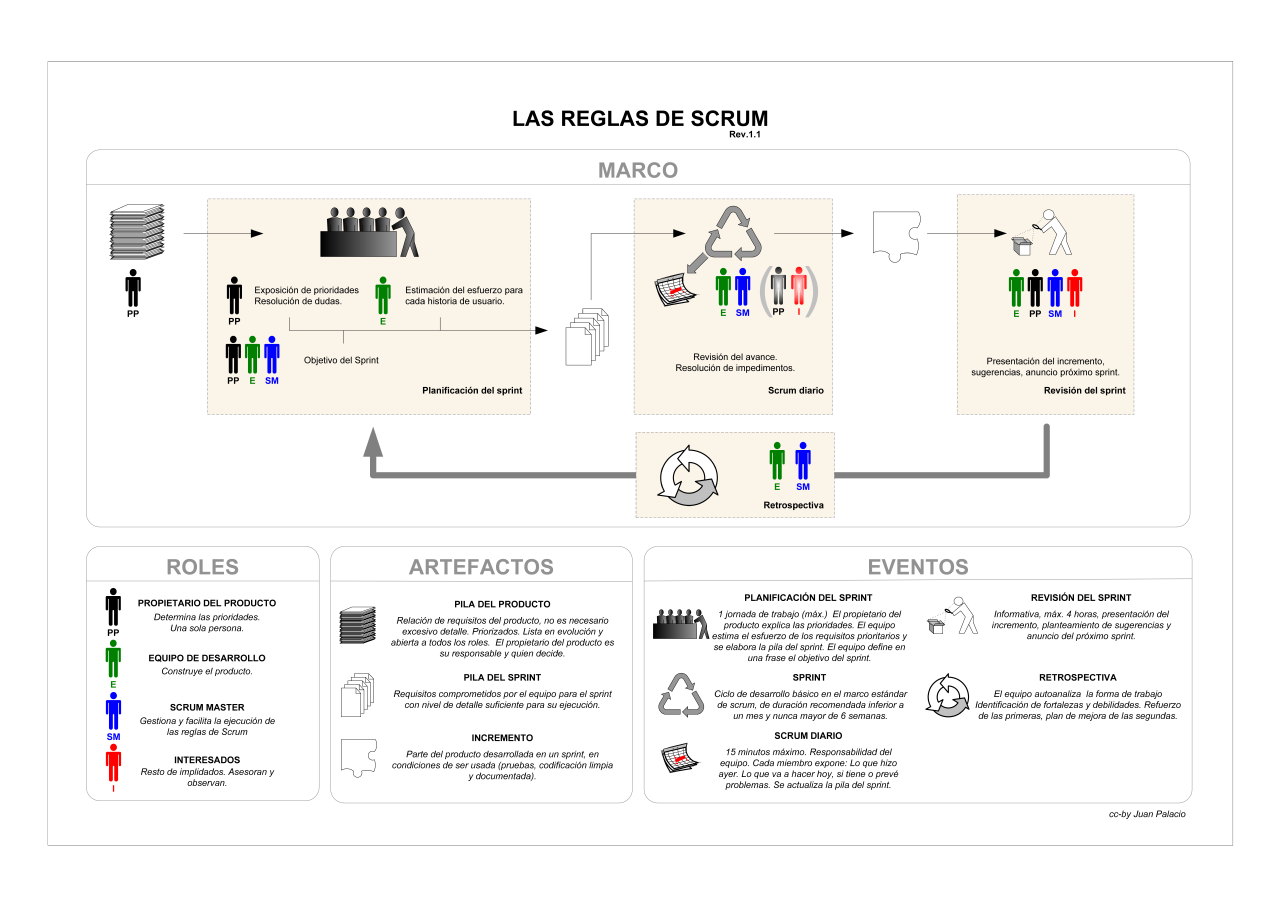
\includegraphics[width=1.2\textwidth]{./img/scrum.png}
		\caption{Reglas de Scrum}
		\label{fig:scrum}
	\end{center}
\end{figure}

\section{Herramientas}

Para la realización de este \acs{TFG} se han utilizado los medios que se presentan a continuación.

\subsection{Hardware}

Para la realización de este TFG se utilizará un ordenador, un móvil Android y un iPhone. El equipo 
necesario ha sido facilitado en su mayoría por Intelygenz.

\begin{itemize}
	\item MacBook Pro Procesador Intel Core i5 @2.5GHz. 8GB RAM 1600 MHz. macOS High Sierra v10.13
	\item Nexus 5x Procesador Qualcomm® Snapdragon™ 808 64 bits, 1.8 GHz, seis núcleos, 2GB RAM con Android 8.1
	\item Nokia 7 Plus Procesador Qualcomm® Snapdragon™ 660 64 bits, 2,2 GHz, ocho núcleos, 4GB RAM con Android 9.0
	\item iPhone 8 Procesador Apple A10 Fusion Quad-Core 64 bits, 2.23 GHz, 2GB RAM con IOS 11
\end{itemize}

\subsection{Software}

 El software necesario para la realización del proyecto es el siguiente:
\begin{itemize}
	\item Android Studio~\cite{ASTUDIO}
	Es el entorno de desarrollo integrado oficial para Android. Se ha utilizado para desarrollar la parte nativa 
	de Android de la aplicación.
	
	\item ECMAScript~\cite{ECMA}~\cite{ECMABOOK}
	
	Es la especificación de un lenguaje de programación, en el cuál se realizará el proyecto.
	
	\item Genymotion
	
	Es un emulador de Android, se ha usado para probar la aplicación en Android.
	
	\item GitHub
	
	
	\item GitKraken
	
	
	\item GitLab Community Edition
	
	
	\item Invision
	
	
	\item IntelliJ IDEA Community~\cite{IDEA}
	
	Para desarrollar la mayor parte de la aplicación.
	
	\item Native Base~\cite{NABA}
	
	Se utilizará para realizar el estilo visual de la aplicación.
	
	\item React Native~\cite{RENA}~\cite{REACTBOOK}
	
	Es el framework que se usa para realizar el desarrollo.
	
	\item Redux~\cite{REDUX}
	
	Para desacoplar el estado global en React Native utilizando el patrón Flux.
	
	\item Slack
	
	
	\item TeXstudio
	
	
	\item Travis
	
	
	\item Xcode~\cite{XCODE}
	
	Para desarrollar la parte nativa de IOS de la aplicación.
\end{itemize}

% Local Variables:
%  coding: utf-8
%  mode: latex
%  mode: flyspell
%  ispell-local-dictionary: "castellano8"
% End:
